\subsection{Query processing}
\subsubsection{Lý thuyết}
\indent Query processing (Xử lý truy vấn) bao gồm các bước hệ thống cơ sở dữ liệu thực hiện để trả về kết quả mong muốn từ một truy vấn của người dùng. Quá trình này bao gồm nhiều bước từ việc phân tích, tối ưu hóa, thực thi và truy xuất kết quả. Các bước chính bao gồm:
\begin{itemize}
    \item Parsing (Phân tích cú pháp): Phân tích cú pháp truy vấn để đảm bảo nó đúng định dạng và cú pháp.
    \item Translation (Biên dịch): Chuyển truy vấn từ ngôn ngữ người dùng sang ngôn ngữ máy có thể hiểu.
    \item Optimization (Tối ưu hóa): Tìm kiếm các kế hoạch thực thi tối ưu để giảm thiểu chi phí và thời gian xử lý.
    \item Execution (Thực thi): Thực hiện kế hoạch truy vấn và truy xuất dữ liệu.
\end{itemize}
\begin{figure}[H]
    \centering
    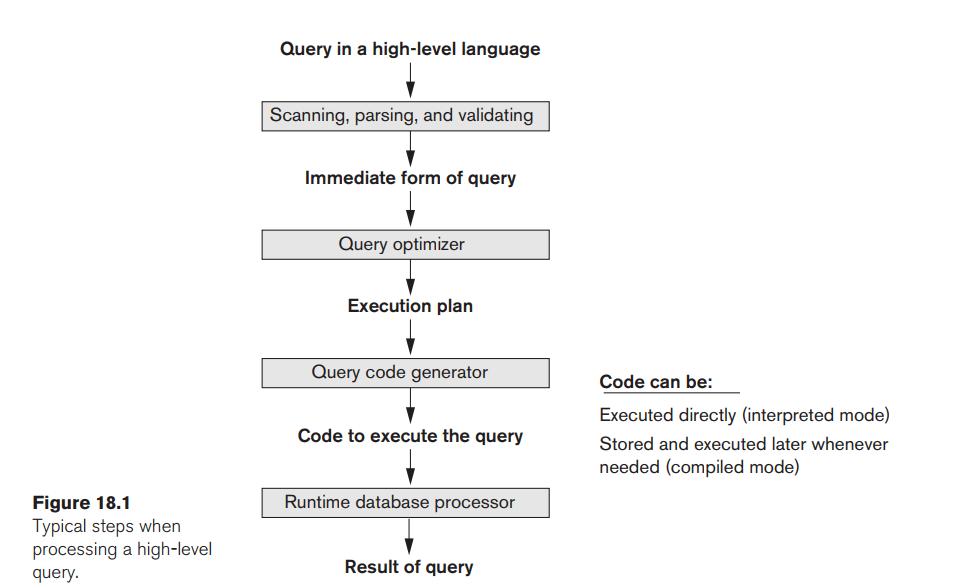
\includegraphics[width=\textwidth]{Image/2.3.1a.png}
    \caption{Các bước khi xử lý truy vấn cấp cao}
\end{figure}
\begin{itemize}
    \item Chi tiết mô tả các bước:
    \begin{itemize}
        \item Query in a high-level language (Truy vấn bằng ngôn ngữ bậc cao): Bắt đầu với một truy vấn được viết bằng ngôn ngữ bậc cao như SQL (trong PostgreSQL) hoặc MQL (trong MongoDB).
        \item Scanning, parsing, and validating (Quét, phân tích cú pháp và xác thực): Truy vấn này sau đó được quét, phân tích cú pháp để đảm bảo nó đúng về cú pháp và ngữ nghĩa.
        \item Immediate form of query (Dạng trung gian của truy vấn): Truy vấn sau khi được xác thực sẽ được chuyển thành dạng trung gian để dễ xử lý hơn.
        \item Query optimizer (Bộ tối ưu hóa truy vấn): Dạng trung gian của truy vấn được chuyển đến bộ tối ưu hóa truy vấn, nơi tạo ra kế hoạch thực thi tối ưu.
        \item Execution plan (Kế hoạch thực thi): Kế hoạch thực thi được tạo ra từ bộ tối ưu hóa.
        \item Query code generator (Bộ tạo mã truy vấn): Kế hoạch thực thi được chuyển đến bộ tạo mã truy vấn.
        \item Code to execute the query (Mã để thực thi truy vấn): Bộ tạo mã truy vấn sẽ tạo ra mã cần thiết để thực thi truy vấn.
        \item Runtime database processor (Bộ xử lý cơ sở dữ liệu runtime): Mã này được thực thi bởi bộ xử lý cơ sở dữ liệu runtime.
        \item Result of query (Kết quả của truy vấn): Cuối cùng, kết quả của truy vấn được trả về.
    \end{itemize}
\end{itemize}

\subsubsection{Query processing trong PostgreSQL}
\indent PostgreSQL sử dụng SQL làm ngôn ngữ truy vấn. Quy trình xử lý truy vấn trong PostgreSQL thường gồm ba bước chính:
\begin{itemize}
    \item Parsing: Phân tích cú pháp truy vấn SQL để tạo cây cú pháp (parse tree).
    \item Planning/Optimization: Sau khi cây cú pháp được tạo ra, PostgreSQL sẽ tiến hành Planning. Bước này sẽ giúp hệ thống quyết định cách thức thực thi truy vấn sao cho hiệu quả nhất. Hệ thống sẽ đánh giá và tạo ra một kế hoạch truy vấn (query plan) với các chiến lược tối ưu như:
        \begin{itemize}
            \item Join Optimization: Nếu có nhiều bảng tham gia vào truy vấn, PostgreSQL sẽ quyết định thứ tự join sao cho tối ưu nhất (sử dụng thuật toán join như Nested Loop, Merge Join, Hash Join).
            \item Index Optimization: Nếu có chỉ mục trên các cột, hệ thống sẽ chọn cách sử dụng các chỉ mục này để tối ưu hóa tìm kiếm thay vì phải quét toàn bộ bảng (full table scan).
            \item Heuristic Methods: Các phương pháp tối ưu hóa theo kinh nghiệm (heuristics) sẽ được áp dụng, như việc sử dụng các thuật toán sắp xếp hoặc kết hợp các chỉ mục.
        \end{itemize}
    \item Execution: Cuối cùng, kế hoạch truy vấn tối ưu sẽ được thực thi bởi executor của PostgreSQL. Executor sẽ thực hiện các phép toán theo kế hoạch đã tối ưu, trả về kết quả cuối cùng cho người dùng. Quá trình này có thể bao gồm quét bảng, áp dụng các phép toán join, và trả về kết quả.
\end{itemize}

\subsubsection{Query processing trong MongoDB}
\indent Mongodb sử dụng MongoDB Query Language (MQL) thay vì SQL. Quy trình xử lý truy vấn trong MongoDB bao gồm ba bước chính:
\begin{itemize}
    \item Parsing: Khi MongoDB nhận được một truy vấn, bước đầu tiên là Parsing, nơi MongoDB sẽ phân tích cú pháp của truy vấn MQL và tạo ra một cây cú pháp tương tự như trong PostgreSQL. Tuy nhiên, MongoDB sử dụng JSON-like documents (tài liệu kiểu JSON) thay vì bảng quan hệ, và truy vấn của MongoDB được cấu trúc dưới dạng các điều kiện như { field: value }.
    \item Planning/Optimization: Sau khi truy vấn được phân tích, MongoDB sẽ tạo ra một query plan. Quá trình tối ưu hóa truy vấn trong MongoDB chủ yếu dựa vào các chỉ mục có sẵn và cấu trúc tài liệu của MongoDB.
        \begin{itemize}
            \item Indexing: Nếu có chỉ mục trên trường age, MongoDB sẽ chọn sử dụng chỉ mục này để tìm kiếm các tài liệu thỏa mãn điều kiện age > 18, thay vì quét toàn bộ bộ sưu tập (collection).
            \item Query Optimization: MongoDB sẽ tối ưu hóa kế hoạch truy vấn để giảm thiểu số lượng tài liệu cần phải quét và cải thiện tốc độ truy vấn.
        \end{itemize}
    \item Execution: Sau khi tạo ra kế hoạch truy vấn tối ưu, MongoDB sẽ thực thi truy vấn đó bằng cách quét các tài liệu trong bộ sưu tập, áp dụng các chỉ mục (nếu có), và trả về kết quả.
\end{itemize}

\subsubsection{So sánh}
\begin{itemize}
    \item Ngôn ngữ truy vấn: PostgreSQL sử dụng SQL, một ngôn ngữ truy vấn quan hệ tiêu chuẩn, trong khi MongoDB sử dụng MongoDB Query Language (MQL), phù hợp với dữ liệu không cấu trúc.
    \item Tối ưu hóa truy vấn: PostgreSQL áp dụng nhiều kỹ thuật tối ưu hóa phức tạp cho các truy vấn SQL, trong khi MongoDB tập trung vào tối ưu hóa dựa trên các chỉ mục và cấu trúc tài liệu.
    \item Thực thi truy vấn: PostgreSQL thực thi kế hoạch truy vấn trên các bảng quan hệ, trong khi MongoDB thực thi trên các tập hợp tài liệu, cho phép xử lý dữ liệu linh hoạt hơn.
\end{itemize}

\begin{table}[H]
    \centering
    \begin{tabular}{|L{3.2cm}|L{5cm}|L{5cm}|} \hline 
         \textbf{Tiêu chí so sánh }&  \textbf{PostgreSQL}&  \textbf{MongoDB}\\ \hline 
         Parsing &  Phân tích cú pháp SQL, tạo cây cú pháp. & Phân tích cú pháp MQL (JSON-like), tạo cây cú pháp.\\ \hline 
         Optimization &  Tối ưu hóa kế hoạch truy vấn sử dụng chỉ mục, thuật toán join, tối ưu hóa biểu thức. & Tối ưu hóa truy vấn dựa vào chỉ mục, cấu trúc tài liệu.\\ \hline 
         Execution &  Thực thi kế hoạch truy vấn, quét bảng hoặc sử dụng chỉ mục. &  Thực thi trên tập hợp tài liệu, xử lý dữ liệu linh hoạt.\\ \hline
    \end{tabular}
    \caption{So sánh về Query Processing PostgreSQL và MongoDB}
    \label{tab:query_processing}
\end{table}
\newpage
